\chapter{Tesztelés}

Az alkalmazás megfelelő működésének érdekében szükséges annak tesztelése.
Ezt manapság mindenhol igyekszenek automatizálni, mivel a manuális tesztelés nem csak időigényes, de sok esetben
repetitív és nagy hibalehetőséggel jár.

Mivel az itt bemutatott szoftver monolitikus, külön a frontendet és backendet nem tartottam célszerűnek tesztelni.

Emiatt az alkalmazáshoz end-to-end (röviden e2e) teszteket írtam, ami a szofver egészét veszi górcső alá, így akár komplex folyamatok
szimulálását is lehetővé teszi.

A következő lépés a megfelelő tesztelési keretrendszer kiválasztása. Az e2e tesztek futtatásához szükség van egy test runner környezetre, egy assertion library-re, valamint egy böngésző emulátorra.

Ezekre a követelményekre sok, egymástól független megoldás létezik, azonban ezek konfigurációja és összekötése nehézkes lehet.
Emiatt döntöttem végül a \lstinline|cypress| könyvtár használata mellett, mely a fent említett funkciókat egyetlen szoftverként
tudja biztosítani.

\begin{lstlisting}[caption=Bejelentkezés tesztelése]
describe("Login flow", () => {
  it("sets auth cookie when logging in via form submission", () => {
    // destructuring assignment of the this.currentUser object
    const user = {
      email: "john@doe.com",
      password: "asdfghjkl",
    }

    cy.visit("/login")

    cy.get("input[name=email]").type(user.email)

    // {enter} causes the form to submit
    cy.get("input[name=password]").type(`${user.password}{enter}`)

    // we should be redirected to /dashboard
    cy.url().should("include", "/")

    // our auth cookie should be present
    cy.getCookie("sess").should("exist")
  })
})
\end{lstlisting}

A tesztek futtatásához először is futnia kell az alkalmazásunknak. Ezután a \lstinline|cypress open| parancs kiadásával
tudjuk megnyitni a futtatókörnyezetet. Itt akár egyesével, akár egymás után tudjuk indítani a tesztjeinket.

\begin{figure}[!ht]
  \centering
  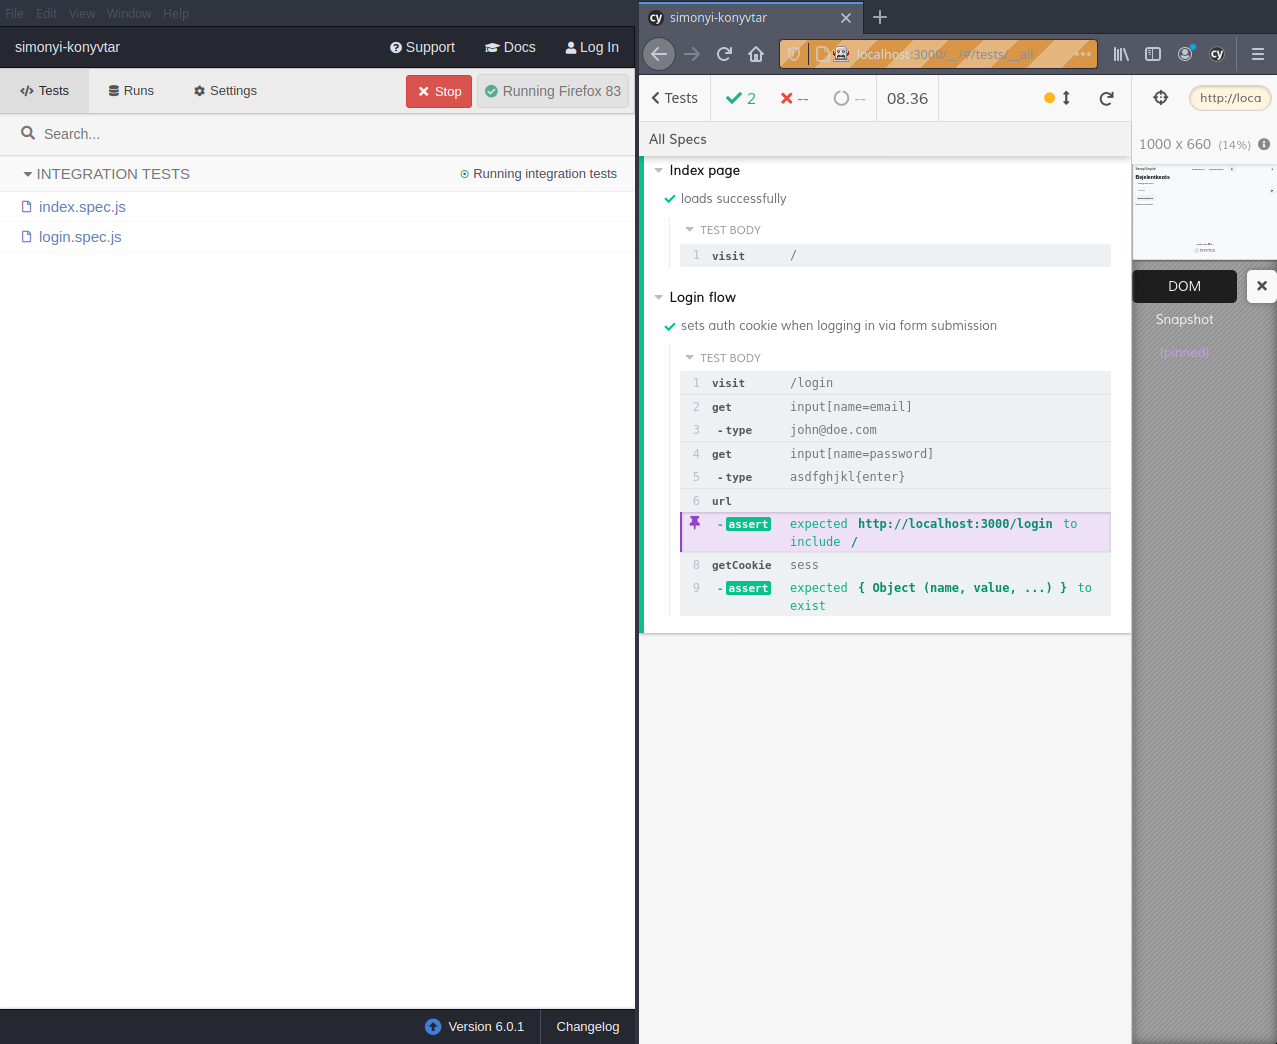
\includegraphics[width=150mm, keepaspectratio]{figures/cypress.png}
  \caption{Tesztek futtatása Cypress segítségével}
  \label{fig:Cypress}
\end{figure}
